% KSe.tex
% $Author$ $Date$

% \section{\KSe}
% \label{s-KS}
% Predrag                    4jul2006
% Predrag                   jun 20 2006
% Vaggelis                  may 20 2006
% extracted from ~dasbuch/book/chapter/PDEs.tex  5jun2005 version
% Predrag                   17sep1999

% \PC{incorporate missing refs from chapter/refsPDEs.tex}

The \KS\ [henceforth KS] system\rf{ku,siv},
which arises in the description of
stability of flame fronts, reaction-diffusion systems and many other
physical settings\rf{KNSks90}, is one of the simplest nonlinear PDEs that
exhibit spatiotemporally chaotic behavior. In the formulation
adopted here, the time evolution of the `flame front velocity'
$u=u(x,t)$ on a periodic domain $u(x,t) = u(x+L,t)$ is given by
\beq
  u_t+{\textstyle\frac{1}{2}}(u^2)_x+u_{xx}+ u_{xxxx}=0
% abandoned the CCP convention: u_t=(u^2)_x-u_{xx}- u_{xxxx}
    \,,\qquad   x \in [0,L]
    \,.
\ee{ks}
Here $t \geq 0$ is the time, and $x$ is the spatial coordinate.
The subscripts $x$ and $t$ denote partial derivatives with respect to
$x$ and $t$. In what follows we use interchangeably the `dimensionless
system size' $\tildeL$, or the periodic domain size $L= 2\pi \tildeL$,
as the system parameter. All numerical results presented in this paper
are for the system size $\tildeL=22/2\pi = 3.5014\dots$.

Spatial periodicity $u(x,t)=u(x+L,t)$
makes it convenient to work in the Fourier space,
\beq
  u(x,t)=\sum_{k=-\infty}^{+\infty} a_k (t) e^{ i k x /\tildeL }
\,,
% \label{fseries}
\ee{eq:ksexp}
%where $\tildeL=L/2\pi$. Thus,
with the $1$-dimensional PDE \refeq{ks}
replaced by an infinite set of
ODEs for the complex Fourier coefficients $a_k(t)$:
\beq
\dot{a}_k= \pVeloc_k(a)
     = ( (k/\tildeL)^2 - ( k/\tildeL)^4 )\, a_k
    - i \frac{k}{2\tildeL} \sum_{m=-\infty}^{+\infty} a_m a_{k-m}
\,.
\ee{expan}
Since $u(x,t)$ is real,
$ %\[
a_k=a_{-k}^*
\,,
$ %\] %\label{cplx-b}
and we can replace the sum in \refeq{expan} by a
sum over $k > 0$.

\PC{find better place for this text?}
Due to the hyperviscous damping $u_{xxxx}$, long time solutions of
\KSe\ are smooth, $a_k$ drop off fast\PC{how fast?} with $k$,
and truncations of \refeq{expan} to $d$ terms, $16 \leq d \leq 128$,
yield highly accurate solutions for system sizes considered here.
Robustness of the Fourier representation of KS as a function of the
number of modes kept in truncations of \refeq{expan} is, however,
a subtle issue.  Adding an extra mode to a truncation of the system
introduces a small perturbation.
However, this can (and often will) throw the dynamics
into a different asymptotic state.
A chaotic attractor for $d=15$ can
collapse into an attractive period-3 cycle for $d=16$, and so on.
\PC{this example is taken from \rf{Christiansen:97}.
    do we have a better one from the current study?
   }
If
we compute, for example, the Lyapunov exponent $\Lyap(\tildeL,d)$ for
a strange attractor of the system \refeq{expan}, there is no reason to
expect $\Lyap(\tildeL,d)$ to smoothly converge to a limit value
$\Lyap(\tildeL,\infty)$ as $d \rightarrow \infty$, because of the lack
of structural stability both as a function of truncation $d$, and the
system size \tildeL.
The topology is more robust for \tildeL\ windows
of transient turbulence, where the system can be structurally stable,
and it makes sense to compute Lyapunov exponents, escape rates, etc.,
for the {repeller}, \ie, the closure of the set of all {unstable}
periodic orbits.

The \eqva\ and short \po s explored in this paper
are robust both under mode truncations and small
system parameter $\tildeL$ changes.
%\PC{Is $L=88.86$ really in \reffig{f:ks_largeL}?}

        \PublicPrivate{%
        }{% switch to Private:
Spatial representations of PDEs (such as the 3$D$
snapshots of velocity and vorticity fields in Navier-Stokes)
offer little insight into detailed dynamics of low-$Re$ flows.
Much more illuminating are the \statesp\ representations.
\PC{expand this into a visualization subsection: how we use
    $d$-dimensional vectors (stability eigenvectors, etc) to project
    from $d$-dimensions to 2 or 3 dimensions. \underline{Not}
    Fourier modes as coordinates!}
        } %end \PublicPrivate{%

%%%%%%%%%%%%%%%%%%%%%%%%%%%%%%%%%%%%%%%%%%%%%%%%%%%%%%%%%%%%%%%%
\begin{figure}[t]
\begin{center}
%\includegraphics[width=0.8\textwidth]{figs/ks_largeL.eps}
\includegraphics[width=0.9\textwidth]{figs/ks_largeL_cbar.eps}
\end{center}
\caption{
A typical `turbulent' solution of the \KSe, system size
$L=20\pi\sqrt{2}\approx 88.86$.  The $x$ coordinate is scaled
with the most unstable wavelength $2\pi\sqrt{2}$, which is
approximately also the mean wavelength of the turbulent flow.
The color bar indicates the color scheme for $u(x,t)$.  This color
scheme is used in other figures of this type throughout this work.
     } \label{f:ks_largeL}
\end{figure}
%%%%%%%%%%%%%%%%%%%%%%%%%%%%%%%%%%%%%%%%%%%%%%%%%%%%%%%%%%%%%%%%%%

\ES{Can we? Galilean invariance allows a rescaling of $a_0$ but
     in \refeq{EFourier} all $a_k$'s appear.}

\subsection{Symmetries of \KSe}
\label{sec:KSeSymm}
% former \subsection{Scaling and symmetries}
% former symm.tex
% Predrag extracted from newton.tex         jul  3 2006

The  KS equation is Galilean invariant: if $u(x,t)$ is a solution,
then $u(x \PCedit{-ct,t) -c} $, with $c$ an arbitrary constant
speed, is also a solution. Without loss of generality, in our
calculations we shall set the mean velocity of the front to zero,
% \index{Galilean invariance}
% \index{invariance!Galilean}
\beq \int dx \, u = 0 \,. \ee{GalInv}
As $\dot{a_0}=0$ in
\refeq{expan}, $a_0$ is a conserved quantity, in our calculations
fixed to $a_0=0$ by the
% Galilean invariance
condition \refeq{GalInv}. The KS equation  \refeq{ks} is time
translationally invariant, and space translationally invariant under
the 1-$d$ Lie group of $O(2)$ rotations: if $u(x,t)$ is a solution,
then $u(x+\shift,t)$ is an equivalent solution for any $-L/2 <
\shift \leq L/2$.
% from newton.tex
The translation operator action on the Fourier coefficients
\beq
  (\mathbf{g}(\shift) a)_k= e^{ik\, \shift /\tildeL}a_k
    \qquad \mbox{(no summation on $k$)}
    \,.
    \label{eq:RPOcondFouri}
\eeq amounts to the $k$-th mode complex plane rotation by an angle
$-k\, \shift /\tildeL$. The KS equation is also invariant under
reflection (`parity' or `inversion')
\beq \Refl u(x) = -u(-x)
\ee{KSparity}
and the shift
\beq \Shift_{1/2} u(x)=u(x+L/2) \,.
\ee{KSshift}
\PCedit{
In the Fourier representation \refeq{expan}
the \Refl\ reflection flips the odd modes,
\beq
a_{2m} \to a_{2m}
    \,,\qquad
a_{2m+1} \to -a_{2m+1}
\,.
\ee{FModInvSymm}
Any rational shift $ \Shift_{1/m}u(x)=u(x+L/m)$
generates a discrete dihedral $D_m$
subgroup of $O(2)$ and is a symmetry of \KS.
In the Fourier representation a solution invariant
under $D_m$ has  only $a_{jm} \neq 0$, $j =1,2,\ldots$
non-zero modes. This observation reduces the dimensionality
of \statesp\ and aids computation of \eqva\ and \po s
within it. However, linearized stability of these solutions has
eigenvectors outside of this subspace, and needs to be
computed in the full \statesp.
    } % \PCedit{
\PC{
    \refeq{FModInvSymm} is probably correct only within the
    the antisymmetric subspace, the complex 1/2-cell translation
    \refeq{eq:RPOcondFouri}
    multiplies modes by $i^k$. \PCedit{RECHECK}
    }
%
% Any \rpo\ of period $\period{p}$ with such rational shift is
% eventually periodic, of period $m\period{p}$. \Rpo s without a
% discrete symmetry have irrational shifts $d$, and are not segments
% of a periodic solution.


Relations $\Refl^2=\Shift_{1/2}^2=1$ induce a linear decomposition
of the space of solutions into 4 invariant subspaces\rf{KNSks90}
    \PCedit{
via four products $\Refl_{1,2} \Shift_{1,2}$ of the
projection operators $\Refl_1=(\matId+\Refl)/2$,
            }
    \PC{this is not as in \refref{KNSks90}, I might be wrong}
$\Refl_2=(\matId-\Refl)/2$, $\Shift_1=(\matId+\Shift_{1/2})/2$, and
$\Shift_2=(\matId-\Shift_{1/2})/2$.  The nonlinear term $(u^2)_x$ in
the KS equation mixes these subspaces, leading
to four invariant subspaces (labeled by the
corresponding projection operators\rf{KNSks90}):
\begin{romannum} % SIAM itemize}
 \item[$\Refl_1$:] The space of antisymmetric functions,
 \item[$\Shift_1$:] The space of $L/2$ periodic functions,
 \item[$\Refl_1 \Shift_1$:] The intersection of the above two,
 \item[$\mathbf{L}$:]
The space of functions invariant under $x\mapsto L/2-x,\ u\mapsto -u$.
\end{romannum} %itemize}

%\subsection{Antisymmetric subspace}
%\label{s:AntisymmSubsp}
%
\KSe\ preserves solutions $u(x,t)=-u(-x,t)$ within the
antisymmetric subspace $\Refl_1$.
With the continuous
translational symmetry eliminated and no
\reqva\ and \rpo s, one
can focus on the \eqva\ and \po s only, as was done
in \refref{Christiansen:97,Lan:Thesis,LanCvi07}.
In the Fourier
representation, the $u$ antisymmetry
amounts to having purely imaginary
coefficients, since $a_{-k}= a^\ast_k = -a_k$.
The 1/2 cell-size shift $\Shift_{1/2}$
generated 2-element discrete subgroup
$\{1,\Shift_{1/2}\}$ is
of particular interest in here,
because in the antisymmetric
subspace the translational invariance of the full system reduces to
invariance under discrete translation \refeq{KSshift} by half a
spatial period $L/2$.

In
this paper we study the full \KS\ system invariant under continuous
translations.
% Due to the lack of self-adjointness (non-normality) of
% the linearized \KS\ flow,
The antisymmetric subspace is unstable
under small perturbations and generic solutions of \KSe\ belong to
the full space. Nevertheless, since, as will be discussed in
\refsect{sec:L22}, the \eqva\ of the KS flow
lie in this subspace, it plays important role for the global
geometry of the flow.

\subsection{\Eqva\ and \reqva} % of the \KSe}
\label{sec:stks}
% former equilibria.tex

% Predrag                   jun 20 2006
% Vaggelis                  may 20 2006
% Predrag                                       05dec2004
% Lan                                           25nov2004
% from Lan thesis                                8jun2004

\Eqva\  (or the steady solutions)
are the simplest flow-invariant solutions,
\beq
 u(x,t) = u_\stagn(x) %\,,\quad t \in \mathbb{R}
\,.
\ee{eqva}
Due to the translational symmetry,
the KS system also allows for \reqv\ solutions
(traveling waves, rotating waves),
characterized by a fixed profile $u_\stagn(x)$
moving with constant speed $c$, {\ie}
\beq
 u(x,t) =  u_\stagn(x-ct) %\,,\quad t \in \mathbb{R}
\,.
\ee{reqva}

Here suffix ${}_\stagn$ labels a particular invariant solution.
Because of the reflection symmetry \refeq{KSparity},
the \reqva\ come in counter-traveling pairs
$u_\stagn(x-ct)$, $-u_\stagn(-x+ct)$. % $c \to -c$.
\Eqva.
%\RLD{Not sure what this means.}
%PC:, OK, dropped now
%and the connections between them form the coarsest
%geometrical framework for organizing
%\statesp\ orbits. %\rf{ksgreene88}.

The \reqv\ condition for the {\KS} PDE \refeq{ks}
is the ODE
\beq
{\textstyle\frac{1}{2}}(u^2)_x+u_{xx}+ u_{xxxx}=c \, u_x
% \,.
\ee{KSeqvCond}
which can be analyzed as a dynamical system in its own right.
\PC{\PCedit{PC: please recheck $E$ vs $c$}}
Integrating once we get
\PC{
    \reqva\ = \eqva\ shifted by $c$?
   }
\beq
{\textstyle\frac{1}{2}}(u-c)^2+u_x+u_{xxx}=\expctE
\,.
\label{eq:stdks}
\eeq
The integration constant \expctE\ can be interpreted as `energy',
see \refsect{sec:energy}.
% Integrate over $L$, and $u_x$, $u_{xx}$ drop put by the
% $L$ periodicity.
Written as a 3-dimen\-si\-on\-al dynamical system
with spatial coordinate $x$ playing the role of `time',
%\refeq{eq:stdks}
this is a volume preserving flow
\beq
\PCedit{
v = -u_x \,,\qquad
w = -v_x \,,\qquad
w_x = {\textstyle\frac{1}{2}}(u-c)^2-v-\expctE
       }
\,,
  \label{eq:3dks}
\eeq
with the `time' reversal symmetry,
\[
x \to -x,\quad u \to -u, \quad v \to v, \quad w \to -w \,.
\]
\PC{might move space average def \refeq{rpo:spac_ave} to here,
    note that
    $\expct{u} = \expct{v} = \expct{w} =0$
    }
 Rewriting \refeq{eq:3dks} as
\beq
\PCedit{
(u+w)_x={\textstyle\frac{1}{2}}(u-c)^2-\expctE
    ={\textstyle\frac{1}{2}}(u-c-\sqrt{2\expctE}) (u-c+\sqrt{2\expctE})
       }
\ee{eqvOfEqv}
we see that
for $\expctE<0$, $u+w$ increases without bound with $x \to \infty$,
and every solution escapes to infinity.
If $\expctE=0$, the origin $(0,0,0)$ is the
only bounded  solution, a marginally stable center with
eigenvalues $(0, i,-i)$.

For $\expctE>0$ there is rich
$\expctE$-dependent dynamics, with
fractal sets of bounded solutions investigated in
depth by Michelson\rf{Mks86}.
The solutions of the {\eqv}  condition
\refeq{eq:3dks} are themselves in turn organized by the
`{\eqva}  of {\eqva}'  condition
\( u_x= v_x= w_x= 0 \), and
the connections between them\rf{Mks86}.
    For $\expctE>0$ the {\reqva}  points of \refeq{eqvOfEqv} are
$C_{+}=(c+\sqrt{2\expctE},0,0)$ and $C_{-}=(c-\sqrt{2\expctE},0,0)$.
Linearization of the flow around $C_{+}$ yields the cubic equation
  \beq
\eigExp(1+\eigExp^2) = 4 \expctE
\,,
  \ee{KSeqvCubic}
with linear stability eigenvalues
\beq
\eigExp[1] = 2 \eigRe
    \,,\qquad
\eigExp[2,3] = - \eigRe \pm i \eigIm
\ee{eqvEqvEigV}
Hence $C_{+}$ has a {1\dmn}
unstable manifold and a 2\dmn\ stable manifold
along which solutions spiral in.
By the $x \to -x$ `time reversal' symmetry, the
invariant manifolds of $C_{-}$
have reversed stability properties.
Most orbits escape quickly even if initiated close to \eqva, and that
renders the numerical calculations
difficult\rf{ksham95,kshooper88,pimyk,pimsimp}.
In this context the variational method
developed in \refrefs{lanVar1,CvitLanCrete02}
appears more robust than
the earlier approaches.


%\subsection{\Eqva\ on a periodic domain}
%

\RLD{This paragraph should probably be moved down after real-space
equation for equilibria and traveling waves are discussed.}
In the Fourier representation the \reqva\ time
dependence is
\beq
 a_k(t) e^{-itc k/\tildeL} = a_k(0)
\,.
\ee{reqvaF}
Differentiating with respect to time, we obtain
the Fourier space version of the \reqv\ condition
\beq
 \pVeloc_k(a) - i \frac{k c}{\tildeL} a_k = 0
\,,
\ee{reqvCondF}
which needs to be solved for (time independent) $a_k$ and $c$.
For a periodic boundary cell of size
$L$ the only {\eqva}  are
solutions of \refeq{eq:3dks} of spatial periodicity $L$.
In the Fourier representation they satisfy
the \eqv\ condition for \refeq{expan}
\beq
\left( \frac{k^2}{\tildeL^2} - \frac{k^4}{\tildeL^4}  \right)\, a_k
    \PCedit{
    -  \frac{i k}{2\tildeL} \sum_{m=-\infty}^{+\infty} a_m a_{k-m}
            }
  = 0
\,.
\label{eq:stfks}
\eeq
Periods of spatially periodic {\eqva} are multiples of $L$.
Every time the system size crosses  $\tildeL=n$,
$n$-cell states
are generated through pitchfork bifurcations off $u =0$
equilibrium.
Due to the translational invariance of {\KSe},
they form invariant circles
in the full \statesp.
In the discrete symmetry subspace considered here,
they correspond to two points, one $L/2$ shift of the other.

For any fixed period $L$ the number
of spatially periodic solutions is finite up to a spatial translation.
For a sufficiently small $L$
the number of {\eqva} is small and
concentrated on the low wave-number end of the Fourier spectrum.

In a periodic box of size $L$
both \eqva\ and \reqva\ are  periodic solutions
embedded in 3-$d$ space \refeq{eq:3dks},
conveniently represented as loops in
$(u,v,w)$ space whose topology is controlled by the
`\eqva\ of \eqva' stable-unstable manifold structure of
\refeq{eqvEqvEigV}, see \reffig{f:KS22Equil}\,(\textit{d}).
In this representation the continuous translation symmetry
is automatic - a rotation in the $[0,L]$ periodic domain only
moves the points along the loop. For an \eqv\ the points
are stationary in time; for \reqv\ they move in time, but in
either case, the loop remains invariant.
So we do not have the problem that we encounter in the Fourier
representation, where from the frame of one of the \eqva\
the rest trace out circles under the action of continuous symmetry
translations.


\subsection{Stability of \eqva}
\label{s:StabEqui}
%%
% Predrag           5jun2005
% extracted from \Chapter{stability}{ 2apr2005}

If $u_\stagn(x)$ is an \eqv\ solution of \KSe,
the {\stabmat}
${\Mvar}={\Mvar}(a_\stagn)$
is constant in time,
and
the {\jacobianM}
of the \eqv\ solution is
\beq
 \jMps^t(a_\stagn) = e^{{\Mvar} t}
    \,,\qquad
 \Mvar_{ij}= \Mvar_{ij}(a_\stagn)
\,.
\ee{eqvFundMat}
Calculation of the {\stabmat} requires a bit of care:
% \refeq{DerMatrix}
$a_{k}$ cannot be varied independently of $a_{-k}$, as
% \refeq{expan}
the reality of $u(x,t)$ implies that $a_{k}=a^*_{-k}$.
We impose the reality constraint by splitting \refeq{expan}
in real and imaginary parts, $a_k=b_k+i\, c_k$. {\Stabmat}
is then:
% \index{Kuramoto-Sivashinsky system}
\bea
    \frac{\partial \dot{c}_k}{\partial c_{j}} & = &
    \frac{k^2}{\tildeL^2}\left(1- \frac{k^2}{\tildeL^2} \right)\delta_{kj}
    - \frac{k}{\tildeL} (c_{k+j}-c_{k-j})
\continue
    \frac{\partial \dot{c}_k}{\partial b_{j}} & = &
    - \frac{k}{\tildeL} ( b_{k+j}+b_{k-j} )
\label{expanMvar}\\
    \frac{\partial \dot{b}_k}{\partial b_{j}} & = &
    \frac{k^2}{\tildeL^2}\left(1- \frac{k^2}{\tildeL^2} \right)\delta_{kj}
    +  \frac{k}{\tildeL} (c_{k+j} + c_{k-j})
\continue
    \frac{\partial \dot{b}_k}{\partial c_{j}} & = &
    - \frac{k}{\tildeL} (b_{k+j}-b_{k-j})
    \,,\qquad  k,j>0
\,.
\nnu
\eea
For the \KSe\ the constant solution $u(x,t)=0$ with zero energy $E$ is an
\eqv\ point of \refeq{ks} which we shall henceforth refer to as
\EQV{0}. For this `laminar' \eqv\ the {\stabmat}
is diagonal, and
so is the {\jacobianM}
$
\jMps^t_{kj}(0) = \delta_{kj} e^{(k/\tildeL)^2(1- (k/\tildeL)^2)t}
\,.
$

The $|k|<\tildeL$
long wavelength perturbations of the flat-front {\eqv}
are linearly unstable, while all
$|k|> \tildeL$ short wavelength perturbations are strongly contractive.
The high $k$ eigenvalues, corresponding to rapid variations of
the flame front, decay so fast that the corresponding eigendirections
are physically irrelevant.
% \index{Lyapunov exponent!{\eqv}}
To illustrate the rapid contraction in the non-leading eigendirections
we plot  in [MAYBE INCLUDE] % \reffig{f:eigenvalues}
the eigenvalues of the \eqv\ in the unstable regime,
for relatively small system size, % low viscosity $\nu$,
and compare them with the
stability eigenvalues of the least unstable cycle for the same
system size.
The `laminar' \EQV{0}~\eqv\ is very unstable,
with many unstable eigendirections.


From \refeq{expan} we see that the origin $u(x,t) = 0$
has Fourier modes as the  linear
stability eigenvectors.
For $0 \leq |k| \leq \tildeL$, these Fourier modes are
unstable.
The most unstable mode, nearest to $|k|=\tildeL/\sqrt{2}$,
sets the scale of the mean wavelength $\sqrt{2}$
of the spatiotemporal dynamics of the {\KSe},
measured in the system size \tildeL, see \reffig{f:ks_largeL}.

Even though our starting point
\refeq{ks}
is an infinite-dimensional dynamical system, the asymptotic dynamics
unfolds on a finite-dimensional attracting manifold, and so we are back on
the familiar territory:
the theory of a finite number of ODEs applies to this
infinite-dimensional PDE as well.

\subsection{Bifurcation structure of \eqva\ and \reqva}
\label{sec:KSlit}
% Vaggelis               jan 20 2007

The \eqva\ of \KSe\ used here are analyzed
in the classical
% bifurcation and symmetry is
papers of
Kevrekidis, Nicolaenko and Scovel\rf{KNSks90},
and Greene and Kim\rf{ksgreene88}. What is new here is
a detailed exploration of the \eqva\ stable/unstable manifolds
for a specific system size $L = 22$, determination
of a large number of \rpo s, and a preliminary
exploration of the relation between the
observed spatiotemporal `turbulent' patterns and
the \rpo s.

In the literature \refeq{ks} is sometimes written as
\beq
    u_t=(u^2)_x-u_{xx}- \nu \, u_{xxxx}
    \,,\qquad   x \in [0,L]
    \,,
\ee{ksVisc}
or in any number of other variants, all equivalent.
The \KSe\ in  form \refeq{ks} is used, among others, by
\cite{cross93,Mks86,ks04com}.
Here we use $L$ as the system parameter, with the
`hyper-viscosity' $\nu$ fixed to $1$.
Other authors vary  $\nu$, with $L$ fixed to either $1$ or $2\pi$.
\PC{remember to mention the scaling of time as well}
In what follows we shall state results of all
calculations either in units of the `dimensionless system size' $\tildeL$,
or the system size $L = 2 \pi \tildeL$. The parameter $\alpha$
of \refrefs{KNSks90,ksgreene88} is in this convention is
$\tildeL=\sqrt{\alpha/4}$.


For small $\tildeL$ the only \eqv\ of the system is the
constant solution $u(x,t)=0$, denoted $\EQV{0}$ here.
$\EQV{0}$ is globally attracting
for $\tildeL<1$. At $\tildeL=n$, $n=1,2,3, \dots$,
the $n$-th harmonic becomes unstable and $\EQV{0}$
undergoes a pitchfork bifurcation into
the antisymmetric `$n$-cell' \eqv, % $\EQV{n}$
together with its $\shift{1/2}$ shift within the
antisymmetric subspace.
For these states the only non-vanishing Fourier coefficients
are $(a_n,a_{2n},\dots)$.
At the system size $\tildeL$ increases, a rich sequence
of bifurcations  follows. The resulting \eqva\ and \reqva\
are identified in \refref{ksgreene88}. For the system size
$L=22$ investigated here, all relevant bifurcations are
summarized by \reffig{fig:ksBifDiag}.

% At point $C$ in \reffig{fig:GreeneKim}
At point $C$ in \reffig{fig:ksBifDiag}
the $2$-cell state bifurcates to a type of \eqv\ solution
found by La Quey, Mahajan, Rutherford and Tang\rf{laquey74}
and generalized by Greene and Kim who refer to them as GLMRT \eqva.
For a GLMRT solution $u(x)$ is antisymmetric,
a long wavelength distorted $n$-cell state.


According to the bifurcation diagram
% \reffig{fig:GreeneKim},
\reffig{fig:ksBifDiag}
and our numerical results,
at the system size $\tildeL=22/2\pi = 3.5014\dots$ studied here,
the {\eqva} are the constant solution \EQV{0},
the GLMRT\rf{laquey74,ksgreene88} \eqv\ \EQV{1},
the $2$- and $3$-cell states \EQV{2} and \EQV{3},
the pair of \reqva\  \REQV{\pm}{1},
and the  \REQV{\pm}{2} \reqva.

%%%%%%%%%%%%%%%%%%%%%%%%%%%%%%%%%%%%%%%%%%%%%%%%%%%%%%%%%%%%%%%%
\begin{figure}[t]       \label{fig:ksBifDiag}
\begin{center}
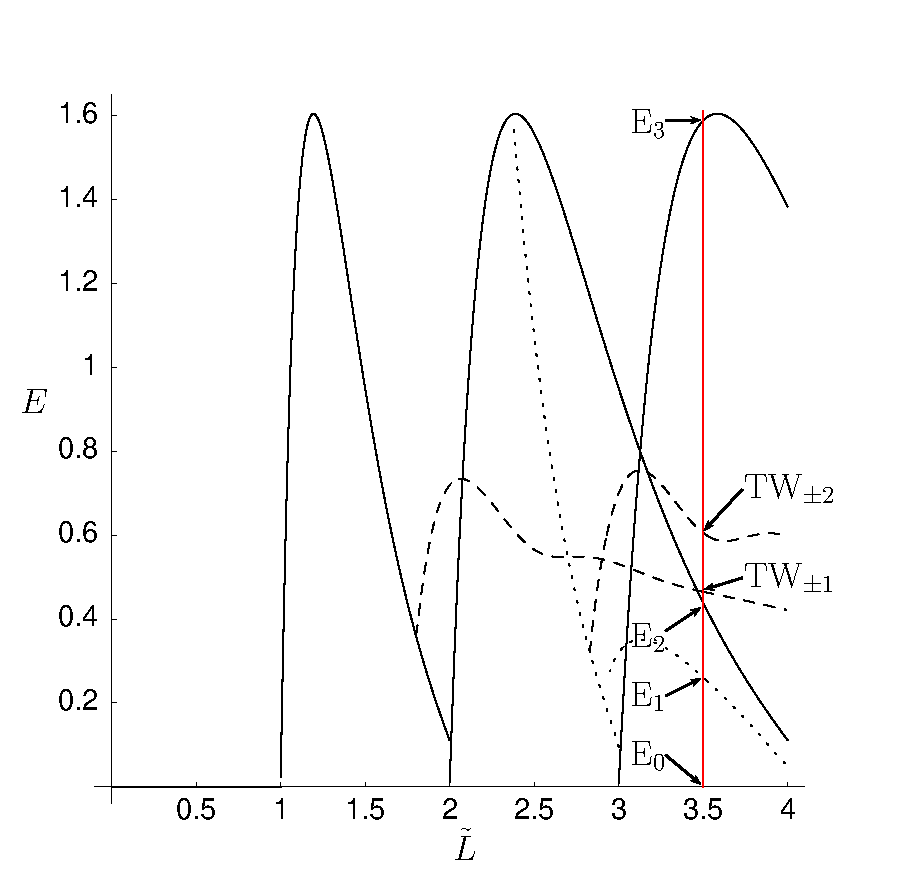
\includegraphics[width=0.5\textwidth]{figs/ksBifDiag_pst.eps}
\end{center}
\caption{
The energy \refeq{ksEnergy}  of all  \eqva\ and \reqva\
that exist up to $L=22$, $\tildeL = 3.5014\ldots$,
plotted as a function of the system size
$\tildeL = L/2\pi$ (additional \eqva, not present at $L = 22$ are
given in \refref{ksgreene88}). Solid curves denote $n$-cell
solutions \EQV{2} and \EQV{3}, dotted curves the GLMRT \eqv\ \EQV{1},
% the dash-dotted curve the `giant states' (??? don't have those),
and
dashed curves the \REQV{\pm}{1},  \REQV{\pm}{2} \reqva.
% Open circles indicate Hopf bifurcations.
%The color of a branch indicates the number of unstable eigenvalues:
%(red) 2 unstable eigenvalues, (blue) 1 unstable eigenvalue, (green)
%stable.
        }
\end{figure}
%%%%%%%%%%%%%%%%%%%%%%%%%%%%%%%%%%%%%%%%%%%%%%%%%%%%%%%%%%%%%%%%%%

\subsection{\Rpo s}
% former history.tex
% Predrag created file              jul 3 2006

The KS equation \refeq{ks} is time translationally invariant,
and space translationally invariant
under the 1-$d$ Lie group of $O(2)$ rotations: if
$u(x,t)$ is a solution, then $u(x+\shift,t)$ is an equivalent
solution for any $-L/2 < \shift \leq L/2$.
As a result, KS can have \reqva\ (traveling wave) solutions
$u(x-ct)$ and \rpo\ solutions with period $\period{}$ and
a nonzero shift $\shift$
\beq
u(x+\shift,\period{}) = u(x,0)
\,,
\ee{KSrpos}
\ie, a state $u(x,0)$ can occur again after time $\period{}$,
but with some shift $\shift$.
Due to the reflection symmetry \refeq{KSparity}, every \rpo\
$u(x,0) = u_\stagn(x)$ with shift $\shift$ has a symmetric partner
$u(x,0) = -u_\stagn(-x)$ with shift $-\shift$.

{\Rpo s} were introduced by Poincar\'e in his study of
the 3-body problem\rf{ChencinerLink,rtb}.
\Reqva\ of this problem are known as the Lagrange points.
% They are stationary in the co-rotating frame, but
% in the inertial frame they execute circular motions.
Our initial searches for \rpo s in KS system were
inspired by Vanessa L{\'o}pez\rf{lop05rel} investigation
of {\rpo s} of the Complex Ginzburg-Landau equation.
{\Rpo s} are periodic orbits in appropriate co-rotating frame,
but in the inertial frame their trajectories
are quasiperiodic.
They arise in dynamics of physical systems
with continuous symmetries, such as motions of rigid bodies, gravitational
$N$-body problems, molecules and nonlinear waves.
For example, Viswanath\rf{ViswanathPC06} % arXiv.org/physics/0604062
has found both \reqva\ and \rpo s in the plane Couette problem.

\subsection{\Po s} \label{sec:KSePO}

If the shift $\shift$ of a \rpo\ with period $\period{}$ is such
that $\shift /L$ is a rational number, then the orbit is
periodic with period $n\period{}$.  As
$\shift$ is continuous in the interval $[-L/2, L/2]$,
the probability to find a \po s is equal to zero,
unless an exact periodicity is enforced by a discrete symmetry.
Due to the \KSe\ invariance
under reflection \refeq{KSparity},
two types of \po s are possible:

{\bf (a)} The \po\ lies within the antisymmetric subspace
$-u(-x,0) = u(x,0)$ and $u(x,\period{}) = u(x,0)$.

{\bf (b) The orbit is reflection symmetric after half
period, $\shift_{1/2} \Refl u(x,0) = -u(L/2-x,0)$.
    \RLD{
    Maybe we should use symmetry operators throughout the discussion?
The general idea is that in chaotic systems with symmetries we should
generalize the notion of a periodic solution from $u(\period{}) = u(0)$
to $u(\period{}) = {\bf S} u(0)$, where ${\bf S}$ is any symmetry
a solution of the system might posses.
\\
PC: good idea
    }
Such orbits, characterized
by the evolution over half the period,
are periodic because orbits starting from
initial conditions related by the reflection symmetry evolve with
opposite shifts, and any shift acquired by the orbit during the evolution
from $0$ to $\period{}/2$ will be compensated by the opposite
shift during evolution from $\period{}/2$ to $\period{}$:
\[
u(x,\period{}) = {\bf R} u(x,\period{}/2) =
   {\bf R}^2 u(x,0) = u(x,0)
   \,.
\]
\Po s built from repetitions of shorter segments
are encountered in any dynamical system with discrete
symmetry\rf{CvitaEckardt,DasBuch}.
